\documentclass{diereport}

\title{Título del documento\footnote{Las opiniones expresadas en este documento representan las de los autores y no necesariamente aquellas del Banco de Guatemala.}}
\author{
  Autor 1\thanks{Autor de correspondencia. Departamento de Investigaciones Económicas, Banco de Guatemala, 7ma. Avenida 22-01 zona 1, Guatemala 01001, Guatemala.}\\
  {\small Banco de Guatemala
  }\\
  {\footnotesize\href{mailto:correo@banguat.gob.gt}{\texttt{correo@banguat.gob.gt}}}
  \and
  Autor 2\\
  {\small Banco de Guatemala}\\
  {\footnotesize\href{mailto:correo@banguat.gob.gt}{\texttt{correo@banguat.gob.gt}}}
%  % Descomentar para más autores
%   \and
%   Autor 3\\
%   {\small Banco de Guatemala}\\
%   {\footnotesize\href{mailto:correo@banguat.gob.gt}{\texttt{correo@banguat.gob.gt}}}
}

% bibliografía
\addbibresource{references.bib}

\begin{document}
	
	% Portada del documento
	\maketitle
	% \vspace*{-2cm}

	% Índice y demás tablas de contenidos
	%\pagenumbering{Roman}
	%\setcounter{page}{2}
	
	\begin{abstract}
	En este documento se investiga el efecto de ...
	\lipsum[10]

	\noindent \textit{JEL classification: E37, E52}.
	\end{abstract}
	
	% Index 
	% \tableofcontents
	
	% Corpus

    % Introduction 
	\section{Introduction}

% Here goes the amazing introduction to the document

According to \textcite[p.~205]{wynne2008core}: ``despite the central role of this concept, there is still no consensus on how best to go about measuring core inflation''; and he adds: ``a common shortcoming is the absence of a well-formulated theory of what these measures of inflation are supposed to be capturing.'' In practice, nevertheless, central banks have developed several ad hoc criteria in order to evaluate, rank and select measures of core inflation.\footnote{See \textcite[p.~9-10]{bankofcanada2021renewal} for a recent application of the most usual criteria for assessing core inflation measures.}

\lipsum[1-2]

	% Literature review
	\section{Review of relevant literature}
\label{section:review_literature}

% In this section we review the current literature body in our research area.

\lipsum[2]
	
	% Methodology
	\section{Methodology}
\label{section:methodology}

% In this section we describe the methodology of our research

En la Figura \ref{figure:awesome_figure} podemos observar que es una gráfica muy bonita.


% Example of illustrative figure
\begin{figure}[htb]
  \caption{The title of our enlightening figure}
  \label{figure:awesome_figure}
  \centering 
  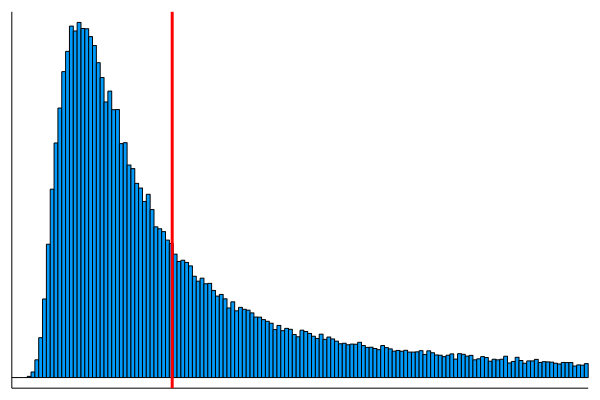
\includegraphics[width=0.9\textwidth]{figures/mse_distribution.png}
  \caption*{\footnotesize Note: error is computed as the standard deviation of the set of realizations... .}
\end{figure}
	
	% Results
	\section{Results}
\label{section:results}

% In this section we describe results

En la Tabla \ref{table:main_results} podemos observar que ...

\lipsum[4]

% We include the main results of the research
\begin{table}[htb]
  \small
  \caption{Main results of the research.}
  \label{table:main_results}
  \begin{tabu} to \textwidth {X[4]X[r]X[r]X[r]X[r]X[r]}
      \toprule
      \textbf{Industry} & Mean & Variance & Covariance & Loss & Simulation Error \\\midrule
      Industry \& Technology                      & 8.6096 & 57.779 & 8.3005 & 74.6892 & 2.1611 \\
      Science \& Health                 & 0.4372 & 0.2117 & 0.4688 & 1.1177 & 0.0014 \\ % Using the CPI formula
      \bottomrule
  \end{tabu}
  \caption*{\footnotesize Note: error is computed as the standard deviation of the set of realizations... .}
\end{table}
		
	% Main findings
	\section{Concluding remarks}
\label{section:concluding_remarks}

	% References
	% \clearpage
	\printbibliography
	
	% Appendix 
	\newpage
	\section*{Appendix}

% In the appendix section we include subsections that detail some procedure or topic within the research document

\renewcommand\thesection{\Roman{section}}
\renewcommand\thesubsection{\Roman{subsection}}
\setcounter{section}{0}
\setcounter{subsection}{0}
\addcontentsline{toc}{section}{Appendix}

% Resetear los contadores de floats
\newcommand{\resetCounters}{
\setcounter{figure}{0}
\setcounter{table}{0}
\setcounter{equation}{0}}

\resetCounters{}

% Change figures, tables, and equations numbering
\renewcommand{\thefigure}{\thesubsection-\arabic{figure}}
\renewcommand{\thetable}{\thesubsection-\arabic{table}}
\renewcommand{\theequation}{\thesubsection-\arabic{equation}}

% Appendix subsections: 
% ------------------------------------

% Formula explanation
\subsection{Formula explanation}
\label{appendix:formula_explanation}

% String literals
\newcommand{\mse}{\text{MSE}(\hat{\pi}^{\star})}
\newcommand{\bias}{\text{Bias}_{\pi}}
\newcommand{\variance}{\text{Var}_\pi}
% Operations
\newcommand{\sumovert}{\sum_{t=1}^{T}}
\newcommand{\meanovert}{\frac{1}{T}\sum_{t=1}^{T}}
% Population parameter and inflation measure
\newcommand{\hatpi}{\hat{\pi}^{\star}}
\newcommand{\barhatpi}{\overline{\hat{\pi}^{\star}}}
\newcommand{\barpi}{\overline{\pi}}
\newcommand{\err}{e}
% Standard errors of parameter and estimator
\newcommand{\spi}{s_{\pi}}
\newcommand{\shatpi}{s_{\hatpi}}
\newcommand{\corr}{r^{\star}}


Consider the error time series $\err_t = \hatpi_t - \pi_t$ for the inflation measure $\hatpi$. Then, $\bias = \meanovert\err_t = \meanovert\hatpi_t - \meanovert\pi_t = \barhatpi-\barpi$. 
First, we show in \ref{eq:mse_is_square_error_plus_bias} that $\mse = \bias^2 + \variance$, where $\variance=\meanovert(\err_t-\bias)^2$ represents the variance of prediction error. This is the classical bias-variance decomposition of the mean square error. 

\begin{equation}
    \begin{aligned}
        \mse & = \meanovert (\hatpi_t - \pi_t)^2\\
        ~ & = \meanovert \left[ (\err_t - \bias) + \bias \right]^2 \\
        ~ & = \meanovert\bias^2 + 2\,\bias\,\meanovert(\err_t-\bias) + \meanovert(\err_t-\bias)^2  \\
        ~ & = \bias^2 + \underbrace{2\,\bias\left(\meanovert\err_t - \meanovert\bias\right)}_{=0} + \meanovert(\err_t-\bias)^2\\
        ~ & = \bias^2 + \variance
    \end{aligned}
    \label{eq:mse_is_square_error_plus_bias}
\end{equation}





\end{document}